\chapter{System zastępowy}
\section{Wstęp}
\begin{wrapfigure}{l}{4cm}
  \begin{center}
    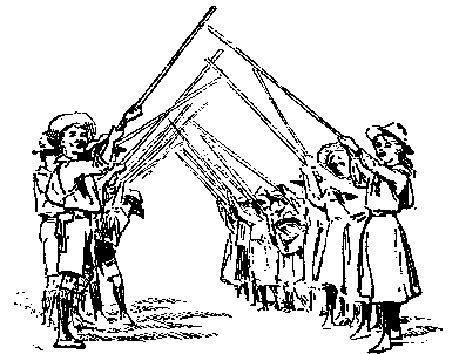
\includegraphics[width=4cm]{grafiki/szpaler.png}
  \end{center}
\end{wrapfigure}Kiedy  spojrzy się na  drużynę, od  razu rzuca  się w  oczy,  że nie jest ona jednolitą całością. 
W każdej grupie liczącej kilkanaście - kilkadziesiąt osób tworzą się  mniejsze  grupki (tak jak np. w  klasie). 
Stworzenie systemu zastępowego, przez Rolanda E. Philipsa było wyjściem na przeciw tworzeniu  się w drużynach właśnie takich małych grupek harcerzy, którzy wybierali sobie jednego spośród nich na przywódcę - zastępowego. 
Chłopcy zawierają  przyjaźnie  ze względu na: wiek, zainteresowania,  miejsce  zamieszkania, chodzenie do jednej klasy. Spełnienie trzech z tych kryteriów może być dobrym kluczem  do stworzenia  solidnego zastępu. 
	
Przy tworzeniu systemu zastępowego w drużynie nie należy nic narzucać, zastępy wytworzą się same, chłopacy sami dobiorą się w grupy, które potem staną  się zastępami. Sztucznie stworzony zastęp nie przejdzie próby czasu (długo się nie utrzyma, a ponadto, ma niewielkie szanse by skutecznie działać).

Gdy w danej grupie (przyszłym  zastępie)  znajduje  się  taki chłopak, który  zawsze ma najwięcej do powiedzenia  i  w  dodatku  pozostali  go  słuchają, wówczas z wyborem zastępowego nie ma problemu. 
Zastępowy powinien dbać o swoich harcerzy z zastępu,  a o rozwój zastępowych dbać powinien drużynowy poprzez prowadzenie zastępu zastępowych (w którym zastępowym jest drużynowy).

Praca zastępu zastępowych  nie powinna znacząco różnić się od pracy poszczególnych zastępów  w  drużynie. Dla wielu zastępowych zbiórki zastępu zastępowych, pod wodzą  drużynowego, mogą być swoistym poligonem doświadczalnym przed zbiórkami  poszczególnych zastępów. Zbiórka zastępu zastępowych na  oczątku tygodnia da możliwość zastępowym powtórzenia jej w  pozostałych dniach już ze  swoimi  zastępami.

System zastępowy nie oznacza tylko, że w drużynie istnieją zastępy, ale że drużynowy prowadzi drużynę przez zastęp zastępowych.

\begin{aquote}{Roland E. Philips}
  System  zastępowy  nie  jest  jedną  z  wielu  metod organizowania  pracy  skautowej, lecz jest  on  jedyną  metodą.
 \end{aquote}
 
 
\section{Zastęp}
\begin{wrapfigure}{l}{3cm}
  \begin{center}
    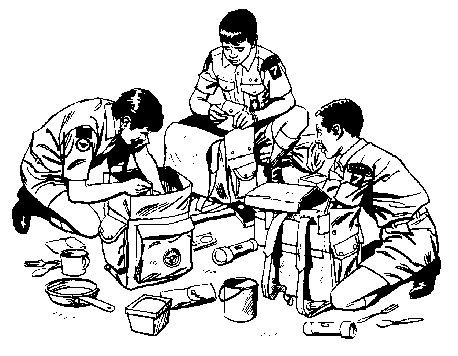
\includegraphics[width=3cm]{grafiki/zastep.png}
  \end{center}
\end{wrapfigure}No, a co to jest ten zastęp? - zastęp jest to grupa chłopców w mniej więcej jednakowym wieku, o tych samych zainteresowaniach i pochodzących z  tego samego środowiska (szkoła - klasa, osiedle - podwórko). 
Liczba  chłopców  w  zastępie  powinna  być około 6 - 8. Pozwala to na dobrą pracę zastępu i oddziaływanie zastępowego  na swoich harcerzy (stopnie, sprawności, zabawa, wykonywanie różnych zadań, wspólne życie obozowe). 
Na czele zastępu stoi zastępowy. 
Jest to chłopiec  o najmniej w tym samym  wieku co członkowie zastępu. Wybija się on spośród nich dzięki swoim zdolnościom przewodzenia w grupie. 
Powinien być wybierany przez zastęp. 
Zastępy mogą być jednopoziomowe, gdy są nim chłopcy w jednym wieku, z jednej akcji naborowej lub wielopoziomowe, gdy co roku, ktoś z zastępu przechodzi do drużyny wędrowniczej, a na jego miejsce dochodzi ktoś nowy.

Pamiętajmy,  że zastęp jest najistotniejszą jednostką naszej organizacji. 
To od zastępu zależy poziom drużyny. 
Każdy zastępowy powinien wiedzieć, że w zastępie wyłaniają się nowe jednostki mogące dalej pozytywnie wpływać  na  rozwój  drużyny.

Silne zastępy to silna organizacja, a silna organizacja to miejsce kształtowania obywateli do  służby dla naszej Ojczyzny.
	
\section{Zastępowy}
Czas teraz zastanowić się, kto to właściwie jest zastępowy. Kim Ty masz być? Zastępowy to ktoś szczególny. To harcerz, który obok drużynowego ma do zrobienia najwięcej w drużynie. Jest to służba, trudna służba, która jednak dobrze wykonywana jest bardzo owocna. \begin{wrapfigure}{r}{4cm}
  \begin{center}
    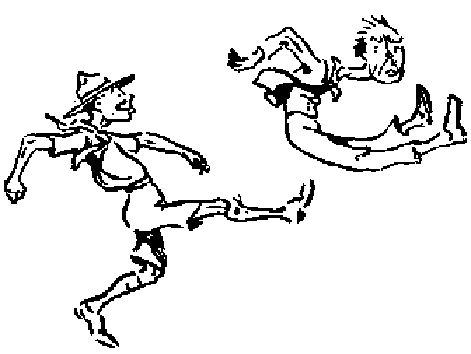
\includegraphics[width=4cm]{grafiki/kop.png}
  \end{center}
\end{wrapfigure} 
	Zastępowy jest jeden a chłopaków wielu. To nieprawda. Zastępowych jest trzech, a wszystko to w jednej osobie.
\begin{itemize}
\item \textbf{Pierwszy zastępowy  to  wzór.}
\item \textbf{Drugi zastępowy to wódz.}
\item \textbf{Trzeci jest  starszym bratem.}
\end{itemize}


Trzy twarze jednego, bardzo ważnego człowieka. Jest wzorem, bo taki, jaki będzie on, tacy będą jego harcerze z zastępu. Wódz - znaczy przewodnik, facet, który ma wśród chłopaków siłę przebicia, słowem odpowiedzialny młody człowiek. Jeżeli zastępowy będzie kumplem, pomocnikiem, opiekunem to będzie starszym bratem. Dzięki tym trzem twarzom zastępowy może samodzielnie prowadzić zastęp i mieć tak wielki wpływ na chłopaków, że może zrobić z nich morowych chłopaków.
	Dobry  wódz musi pamiętać o tym, że niezbędna jest praca ze wszystkimi  harcerzami  ze  swojego  zastępu. Tylko dzięki takiej pracy będą najlepsi.  Tylko wówczas, gdy będą razem zdobędą szczyty.
	Zastępowy koniecznie chce być w swojej pracy najlepszy. Tu objawia się zastępowy - wzór. Musi pokazać swojemu zastępowi, że potrafi  słuchać i wykonywać rozkazy bez względu na to, czy jest obecny  drużynowy czy nie. Nieodzowne jest przodowanie zastępowego w zdobywaniu stopni i sprawności. Zastępowy - wzór sprawdza się w każdych warunkach i dlatego chłopcy pójdą za nim bez zbędnych tłumaczeń.

Nie można jednak zapomnieć, że (jak pisał Robert Baden - Powell): musicie nimi kierować a nie popychać ich. 

\noindent
Pamiętajcie także, że zastępowy:
\begin{itemize}\itemsep1pt

\item znawca technik harcerskich
\item  świeci przykładem: styl harcerski, pogoda ducha, nauka, dom, kultura, pomoc bliźnim
\item  dba o wszystko w  zastępie:  począwszy od  tego czy jego harcerze noszą pas  w szlufkach, przez tworzenie nowych gier, wyjazdy na wycieczki, czy biwaki, aż do zdobywania sprzętu na obozy.
\item  prowadzi zastęp wg planu, który wymyślił wraz zastępem - pisze więc mądry plan działania i konsekwentnie go realizuje, aż osiągnie cel. Prowadzi też książkę lub zeszyt zastępowego (nie na  pokaz  tylko dla samego  siebie), gdzie ma listę swoich harcerzy, notatki o nich, sieć alarmową, plan działania, plany zbiórek, comiesięczny rachunek sumienia (co się udało a co nie), decyzje Rady Zastępu i Rady Drużyny i wszystko co jeszcze jest mu potrzebne w pracy zastępu.
\item  zna i wciąż poznaje: problemy, zdolności, zainteresowania, niepowodzenia itp. swoich harcerzy z zastępu.
\item   widzi, że każdy chłopiec z zastępu jest inny: zastęp to nie szara masa identycznych chłopaków, jeśli to zacznie dostrzegać to będzie wiedział,  że  z każdym chłopakiem trzeba pracować osobno.
\item  uczy chłopaków odpowiedzialności za siebie i  innych.
\item  nie jest dla harcerzy kapralem i ograniczeniem, lecz pociąga ich za sobą.
\end{itemize}

I jeszcze jedno:
\begin{aquote}{Hm. P. Stawiński HR}
Zastępowy  nosi  głowę  w chmurach, ale  nogami  mocno  stąpa  po  ziemi.
 \end{aquote}



\section{Duchowość zastępowego}

Zastanawiasz się czasem, czy harcerz to ktoś wierzący w Boga? – tak, to ktoś właśnie taki. Co więcej, harcerz to wzór życia duchowego, moralności – sami wiecie jak często jest z tym u nas trudno. Tym większa rola zastępowego.

W wielu domach rodzice nie przekazują już wiary, nie jest ona silna. Ty masz za zadanie być wówczas kimś, kto kieruje także duchowości swojego zastępu. Twój zastęp, to taki mały Kościół, który został przez Boga powierzony właśnie Tobie. Powinieneś dbać o to, czy chłopcy chodzą do Kościoła, do spowiedzi, czy się modlą, robią rachunek sumienia, czy starają się być lepsi każdego dnia. Wiadomo, nie można ich do tego zmuszać, ale zachęcać. \begin{wrapfigure}{r}{3cm}
  \begin{center}
    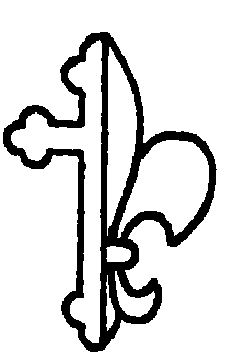
\includegraphics[width=3cm]{grafiki/duchowosc.png}
  \end{center}
\end{wrapfigure} W jaki sposób? – proste, przykładem własnym. Kiedy Ty będziesz się modlił, uczestniczył we Mszy św., kiedy będziesz lektorem i będziesz dobrym człowiekiem, oni bardzo szybko zapragną być tacy jak Ty. Wówczas szybko staną obok Ciebie przy ołtarzu, czy w kolejce do konfesjonału. Widzisz jakie to proste. Proszę też, abyś czasem modlił się za swoich chłopców w zastępie, drużynowego, to także wielka dla nich pomoc. Nie zapomnij też, ze masz obok kapelana, który może Ci zawsze pomóc.

Na obozie zaś nie zapominaj o modlitwie porannej, wieczornej, przed posiłkami, po nich, o Mszy św., o wieczornym rachunku sumienia i o tym, że Bóg jest gdzieś blisko, może nawet w drugim człowieku\ldots